%
% 04001-signal.tex -- 
%
% (c) 2019 Prof Dr Andreas Müller, Hochschule Rapperswil
%
\documentclass[tikz]{standalone}
\usepackage{amsmath}
\usepackage{times}
\usepackage{txfonts}
\usepackage{pgfplots}
\usepackage{csvsimple}
\usetikzlibrary{arrows,intersections,math}
\begin{document}

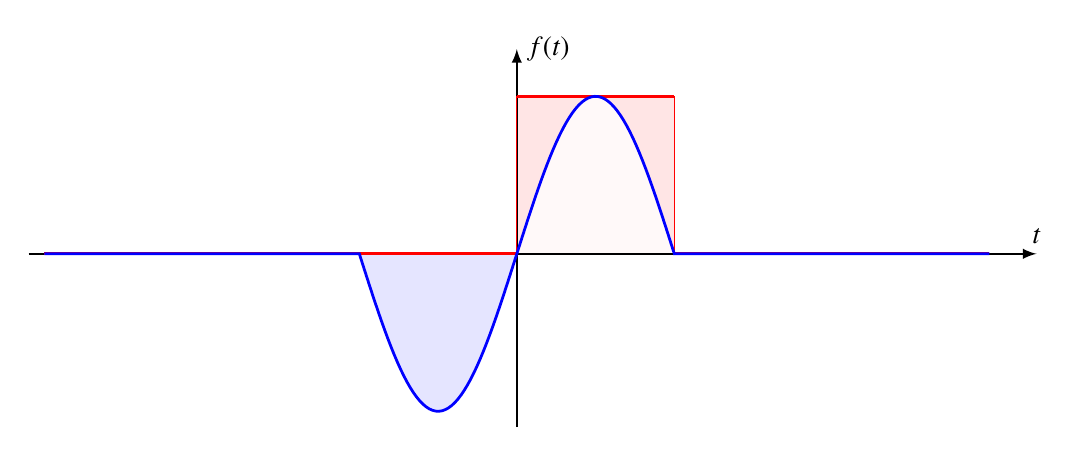
\begin{tikzpicture}[>=latex,scale=2]
\fill[color=red!10] (0,0)--(1,0)--(1,1)--(0,1)--cycle;
\fill[color=pink!10] plot[domain=0:180,samples=100] ({\x/180},{sin(\x)})--cycle;
\fill[color=blue!10] plot[domain=-180:0,samples=100] ({\x/180},{sin(\x)})--cycle;
\draw[->,line width=0.7pt] (-3.1,0)--(3.3,0) coordinate[label={$t$}];
\draw[->,line width=0.7pt] (0,-1.1)--(0,1.3) coordinate[label={right:$f(t)$}];
\draw[line width=1pt,color=red] (-3,0)--(0,0);
\draw[line width=0.3pt,color=red] (0,0)--(0,1);
\draw[line width=1pt,color=red] (0,1)--(1,1);
\draw[line width=0.3pt,color=red] (1,0)--(1,1);
\draw[line width=1pt,color=red] (1,0)--(3,0);

\draw[color=blue,line width=1pt] (-3,0)--
	plot[domain=-180:180,samples=100] ({\x/180},{sin(\x)})
	--(3,0);
\end{tikzpicture}
\end{document}
